\documentclass[14pt]{extbook}
\usepackage{multicol, enumerate, enumitem, hyperref, color, soul, setspace, parskip, fancyhdr} %General Packages
\usepackage{amssymb, amsthm, amsmath, latexsym, units, mathtools} %Math Packages
\everymath{\displaystyle} %All math in Display Style
% Packages with additional options
\usepackage[headsep=0.5cm,headheight=12pt, left=1 in,right= 1 in,top= 1 in,bottom= 1 in]{geometry}
\usepackage[usenames,dvipsnames]{xcolor}
\usepackage{dashrule}  % Package to use the command below to create lines between items
\newcommand{\litem}[1]{\item#1\hspace*{-1cm}\rule{\textwidth}{0.4pt}}
\pagestyle{fancy}
\lhead{Progress Quiz 6}
\chead{}
\rhead{Version C}
\lfoot{9689-6866}
\cfoot{}
\rfoot{Spring 2021}
\begin{document}

\begin{enumerate}
\litem{
Solve the rational equation below. Then, choose the interval(s) that the solution(s) belongs to.\[ \frac{-4x}{-4x -7} + \frac{-6x^{2}}{-16x^{2} -8 x + 35} = \frac{5}{4x -5} \]\begin{enumerate}[label=\Alph*.]
\item \( x \in [0.45,1.44] \)
\item \( x_1 \in [-0.73, 0.32] \text{ and } x_2 \in [0.46,9.46] \)
\item \( \text{All solutions lead to invalid or complex values in the equation.} \)
\item \( x_1 \in [-0.73, 0.32] \text{ and } x_2 \in [-8.75,-0.75] \)
\item \( x \in [2.33,3.1] \)

\end{enumerate} }
\litem{
Determine the domain of the function below.\[ f(x) = \frac{4}{30x^{2} +2 x -12} \]\begin{enumerate}[label=\Alph*.]
\item \( \text{All Real numbers except } x = a, \text{ where } a \in [-27, -22] \)
\item \( \text{All Real numbers except } x = a, \text{ where } a \in [-0.67, 0.33] \)
\item \( \text{All Real numbers except } x = a \text{ and } x = b, \text{ where } a \in [-27, -22] \text{ and } b \in [11, 17] \)
\item \( \text{All Real numbers except } x = a \text{ and } x = b, \text{ where } a \in [-0.67, 0.33] \text{ and } b \in [0.6, 2.6] \)
\item \( \text{All Real numbers.} \)

\end{enumerate} }
\litem{
Choose the graph of the equation below.\[ f(x) = \frac{1}{(x + 1)^2} - 3 \]\begin{enumerate}[label=\Alph*.]
\begin{multicols}{2}\item 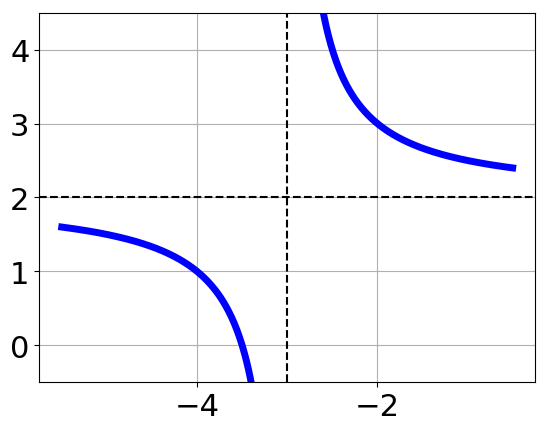
\includegraphics[width = 0.3\textwidth]{../Figures/rationalEquationToGraphAC.png}\item 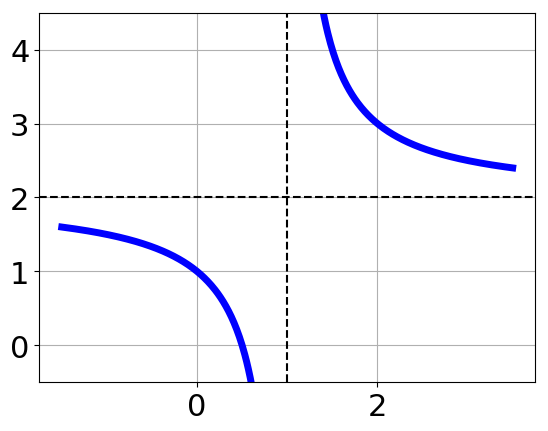
\includegraphics[width = 0.3\textwidth]{../Figures/rationalEquationToGraphBC.png}\item 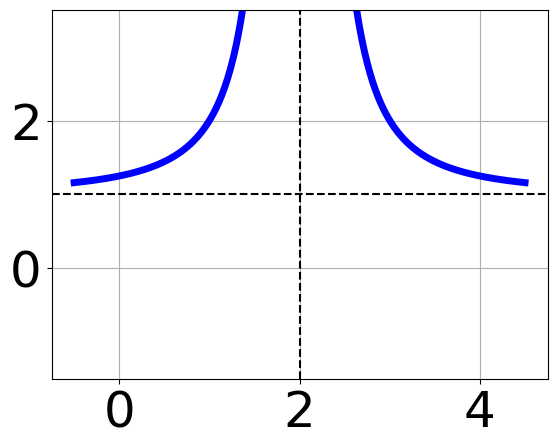
\includegraphics[width = 0.3\textwidth]{../Figures/rationalEquationToGraphCC.png}\item 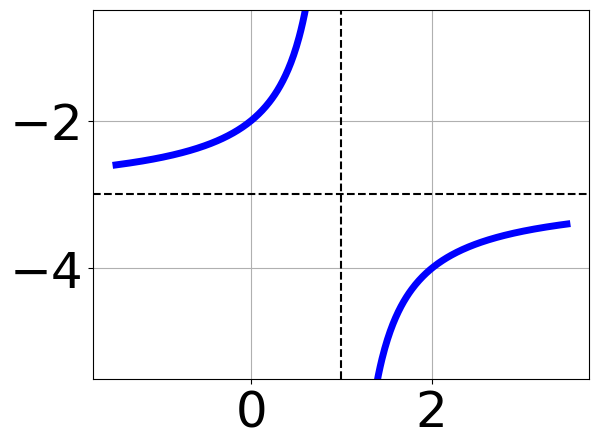
\includegraphics[width = 0.3\textwidth]{../Figures/rationalEquationToGraphDC.png}\end{multicols}\item None of the above.
\end{enumerate} }
\litem{
Choose the graph of the equation below.\[ f(x) = \frac{-1}{x - 3} - 1 \]\begin{enumerate}[label=\Alph*.]
\begin{multicols}{2}\item 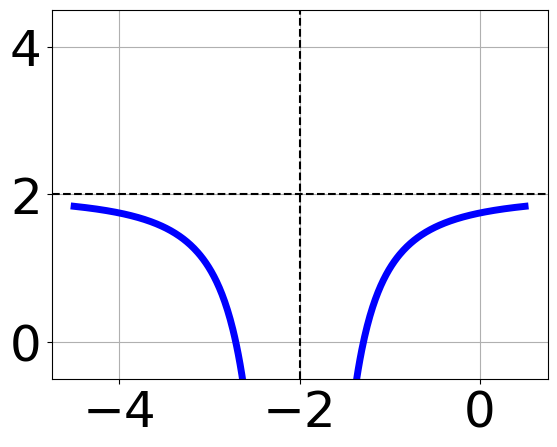
\includegraphics[width = 0.3\textwidth]{../Figures/rationalEquationToGraphCopyAC.png}\item 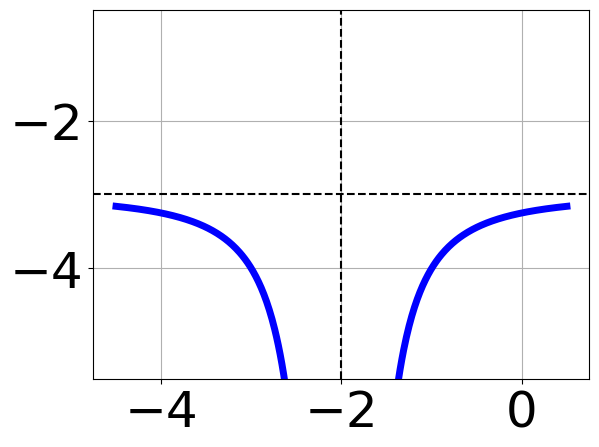
\includegraphics[width = 0.3\textwidth]{../Figures/rationalEquationToGraphCopyBC.png}\item 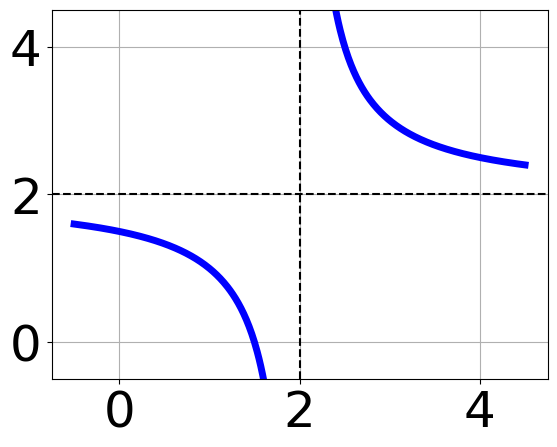
\includegraphics[width = 0.3\textwidth]{../Figures/rationalEquationToGraphCopyCC.png}\item 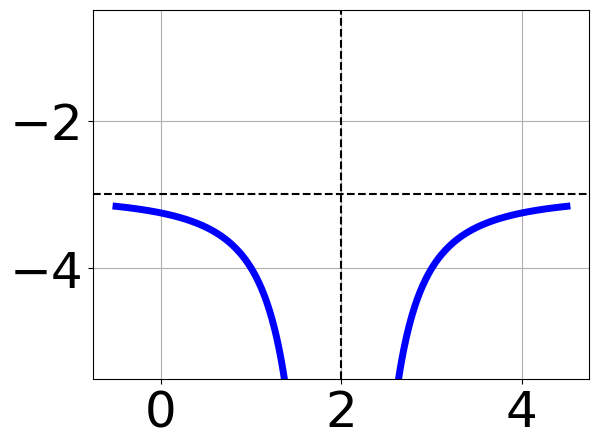
\includegraphics[width = 0.3\textwidth]{../Figures/rationalEquationToGraphCopyDC.png}\end{multicols}\item None of the above.
\end{enumerate} }
\litem{
Choose the equation of the function graphed below.
\begin{center}
    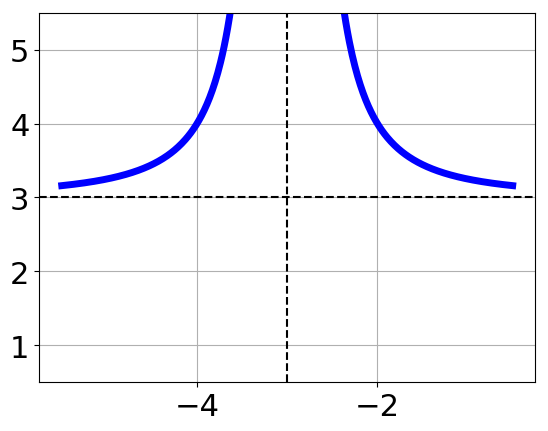
\includegraphics[width=0.5\textwidth]{../Figures/rationalGraphToEquationC.png}
\end{center}
\begin{enumerate}[label=\Alph*.]
\item \( f(x) = \frac{-1}{(x - 1)^2} - 2 \)
\item \( f(x) = \frac{-1}{x - 1} - 2 \)
\item \( f(x) = \frac{1}{x + 1} - 2 \)
\item \( f(x) = \frac{1}{(x + 1)^2} - 2 \)
\item \( \text{None of the above} \)

\end{enumerate} }
\litem{
Choose the equation of the function graphed below.
\begin{center}
    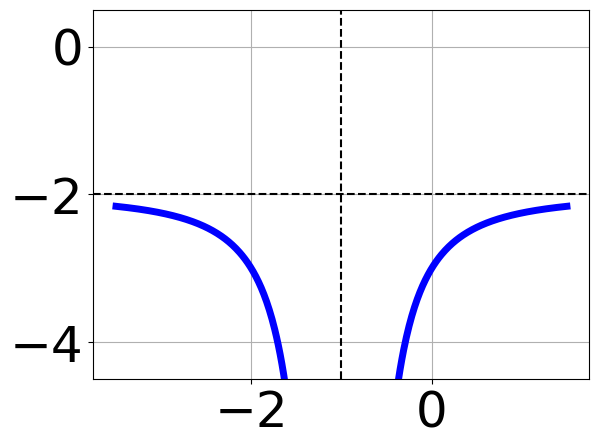
\includegraphics[width=0.5\textwidth]{../Figures/rationalGraphToEquationCopyC.png}
\end{center}
\begin{enumerate}[label=\Alph*.]
\item \( f(x) = \frac{-1}{(x - 3)^2} + 3 \)
\item \( f(x) = \frac{-1}{x - 3} + 3 \)
\item \( f(x) = \frac{1}{(x + 3)^2} + 3 \)
\item \( f(x) = \frac{1}{x + 3} + 3 \)
\item \( \text{None of the above} \)

\end{enumerate} }
\litem{
Solve the rational equation below. Then, choose the interval(s) that the solution(s) belongs to.\[ \frac{-4}{-2x -2} + -2 = \frac{4}{16x + 16} \]\begin{enumerate}[label=\Alph*.]
\item \( x_1 \in [-2.12, 0.88] \text{ and } x_2 \in [1.8,2.1] \)
\item \( x_1 \in [-2.12, 0.88] \text{ and } x_2 \in [-0.4,1.6] \)
\item \( x \in [-0.12,0.88] \)
\item \( \text{All solutions lead to invalid or complex values in the equation.} \)
\item \( x \in [0.88,2.88] \)

\end{enumerate} }
\litem{
Solve the rational equation below. Then, choose the interval(s) that the solution(s) belongs to.\[ \frac{126}{-84x -126} + 1 = \frac{126}{-84x -126} \]\begin{enumerate}[label=\Alph*.]
\item \( x_1 \in [-1.5, 0.5] \text{ and } x_2 \in [-1.5,0.5] \)
\item \( \text{All solutions lead to invalid or complex values in the equation.} \)
\item \( x \in [-0.5,3.5] \)
\item \( x_1 \in [-1.5, 0.5] \text{ and } x_2 \in [1.5,2.5] \)
\item \( x \in [-1.5,0.5] \)

\end{enumerate} }
\litem{
Solve the rational equation below. Then, choose the interval(s) that the solution(s) belongs to.\[ \frac{-6x}{-7x + 7} + \frac{-6x^{2}}{-42x^{2} +7 x + 35} = \frac{-5}{6x + 5} \]\begin{enumerate}[label=\Alph*.]
\item \( x \in [-2.21,-1.95] \)
\item \( x \in [-1.41,-0.27] \)
\item \( x_1 \in [-0.13, 0.94] \text{ and } x_2 \in [1,7] \)
\item \( x_1 \in [-0.13, 0.94] \text{ and } x_2 \in [-4.97,-0.97] \)
\item \( \text{All solutions lead to invalid or complex values in the equation.} \)

\end{enumerate} }
\litem{
Determine the domain of the function below.\[ f(x) = \frac{5}{24x^{2} -6 x -30} \]\begin{enumerate}[label=\Alph*.]
\item \( \text{All Real numbers except } x = a, \text{ where } a \in [-36.7, -35.4] \)
\item \( \text{All Real numbers except } x = a \text{ and } x = b, \text{ where } a \in [-36.7, -35.4] \text{ and } b \in [19.3, 20.3] \)
\item \( \text{All Real numbers except } x = a, \text{ where } a \in [-1.2, -0.4] \)
\item \( \text{All Real numbers except } x = a \text{ and } x = b, \text{ where } a \in [-1.2, -0.4] \text{ and } b \in [0.5, 1.8] \)
\item \( \text{All Real numbers.} \)

\end{enumerate} }
\end{enumerate}

\end{document}